\section{Árbol sintáctico}

\subsection{Representación elegida}

Para toda entrada válida el parser construye un \textbf{árbol sintáctico (árbol de derivación)}: cada nodo interno corresponde a un no terminal de la gramática y cada hoja a un terminal (token) o a $\varepsilon$. Elegimos el árbol de derivación y no un AST reducido porque así se puede comprobar directamente, producción por producción, que el parser siguió la gramática de la sección 3.2.

El árbol se construye mientras se analiza: cada método del parser crea un \texttt{Nodo} para su no terminal y le agrega como hijos los nodos de lo que consume. La clase \texttt{Nodo} (archivo \texttt{arbol.py}) guarda el símbolo, el token asociado (solo en las hojas) y la lista de hijos.

\subsection{Formatos de salida}

El módulo \texttt{arbol.py} ofrece dos formas de visualizar el árbol:

\begin{itemize}
    \item \textbf{Texto jerárquico} (\texttt{imprimir\_arbol}): se muestra en la terminal con caracteres de árbol. Las hojas de tipo \texttt{ID}, \texttt{NUM} y \texttt{OP\_REL} muestran también su lexema (por ejemplo \texttt{ID: vida}). Por defecto se ocultan los nodos $\varepsilon$ para que el árbol sea más legible; la opción \texttt{--epsilon} los muestra.
    \item \textbf{Graphviz} (\texttt{exportar\_dot}): genera un archivo DOT con los no terminales como elipses y los terminales como cajas azules. Se obtiene con \texttt{python main.py -f ejemplos/arbol.gr --dot arbol.dot} y se convierte a imagen con \texttt{dot -Tpng arbol.dot -o arbol.png}.
\end{itemize}

\subsection{Ejemplo}

Para la entrada \texttt{WHEN NOT escudo THEN activar escudo(10);}, que usa la extensión de \texttt{NOT} y las acciones con parámetros, el programa produce el siguiente árbol (sin nodos $\varepsilon$):

\begin{lstlisting}
<programa>
|-- <regla>
|   |-- WHEN
|   |-- <condicion>
|   |   |-- <termino>
|   |   |   |-- <factor>
|   |   |   |   |-- NOT
|   |   |   |   `-- <factor>
|   |   |   |       |-- ID: escudo
|   |   |   |       `-- <comparacion>
|   |   |   `-- <termino'>
|   |   `-- <condicion'>
|   |-- THEN
|   |-- <accion>
|   |   |-- ID: activar
|   |   |-- <objeto>
|   |   |   `-- ID: escudo
|   |   `-- <parametros>
|   |       |-- (
|   |       |-- <argumentos>
|   |       |   |-- <valor>
|   |       |   |   `-- NUM: 10
|   |       |   `-- <argumentos'>
|   |       `-- )
|   `-- ;
`-- <programa'>
\end{lstlisting}

(En la terminal el programa dibuja las ramas con caracteres de línea; aquí se reemplazaron por texto simple.) Se pueden leer en el árbol las decisiones de la gramática: el \texttt{NOT} y su operando están bajo un mismo \texttt{<factor>}, la acción tiene verbo (\texttt{activar}), objeto (\texttt{escudo}) y un parámetro (\texttt{10}), y los nodos \texttt{<termino'>}, \texttt{<condicion'>}, \texttt{<comparacion>} y \texttt{<argumentos'>} aparecen sin hijos visibles porque derivaron $\varepsilon$.

\subsection{Árbol de la regla con AND y NOT}

La figura siguiente muestra el árbol de la regla \texttt{WHEN vida < 20 AND NOT jefe\_cerca THEN usar pocion(1);}, generado con Graphviz. Se aprecia cómo el \texttt{AND} queda dentro de \texttt{<termino'>}, es decir, a un nivel de precedencia mayor que el \texttt{OR}.

\begin{figure}[H]
\centering
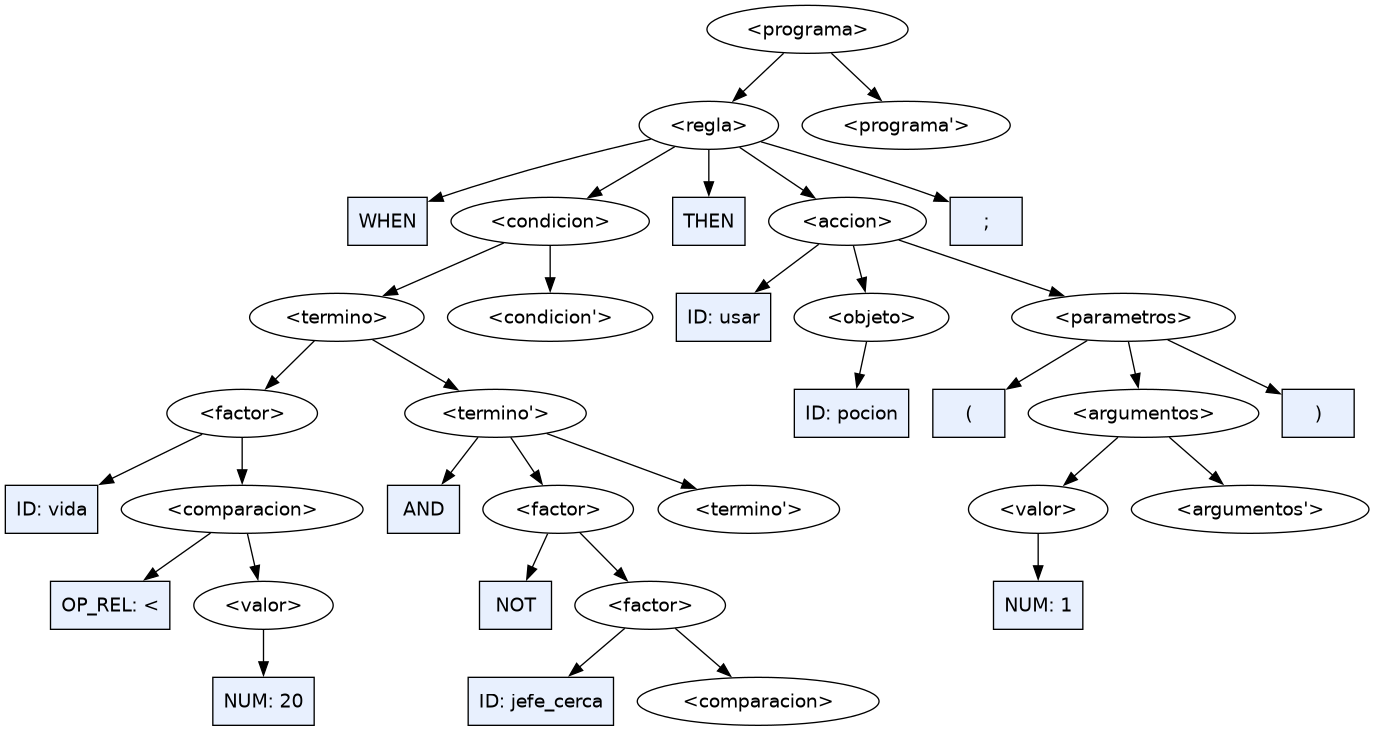
\includegraphics[width=\textwidth]{arbol.png}
\caption{Árbol sintáctico de \texttt{WHEN vida < 20 AND NOT jefe\_cerca THEN usar pocion(1);}.}
\end{figure}

\newpage
